
\begin{table}[t]
\begin{minipage}{.45\linewidth}
\begin{center}
\resizebox{\textwidth}{!}{
 \begin{tabular}{||p{1.3cm}| p{2cm}|} 
 \hline
  \textbf{Hardware}  & \textbf{Configuration}\\
 \hline
 \textit{CPU}  & Xeon E5-2670 \\
 \hline
 \textit{Cores} & 12x2(threads) \\  
  \hline
  \textit{Clock} & 2.3 Ghz \\
  \hline
  \textit{DRAM} & 192 GB \\
  \hline
  \textit{GPU} &  P100(16GB) \\
  \hline
%   \textit{GPU2} & K80(12GB)x2 \\
%   \hline 

  \end{tabular}}
\end{center}

\caption{Hardware config}
\label{tbl:hw-config}

\end{minipage}%
 \hspace{2mm}
\begin{minipage}{.45\linewidth}
\begin{center}

 \resizebox{\textwidth}{!}{%
 \begin{tabular}{|p{1.8cm}| p{2cm} ||} 
 \hline
   \textbf{Software} & \textbf{Version} \\
   \hline
   \textit{Kubernetes} & 1.9.3 \\ 
%    \hline
%    \textit{Docker} &  2.9 \\ 
   \hline
   \textit{NvidiaDocker} &  2.0 \\
   \hline
   \textit{pyNVML} & 7.352.0 \\ 
   \hline
   \textit{InFluxDB} & 1.4.2  \\ 
   \hline
   \textit{CUDA} & 8.0.61 \\ 
   \hline
   \textit{Tensorflow} &  1.8 \\
  \hline
\end{tabular}}
\end{center}

\caption{Software config}
\label{tbl:sw-config}
\end{minipage}%
\end{table}
% \vspace{-0.1in}
\subsection{Experimental setup}
%\begin{itemize}
%\item{\textbf{Hardware:}}
\subsubsection{Hardware}

We use Dell PowerEdge R730 eleven node cluster where ten worker nodes have P100 GPUs with Intel Xeon CPU host along with a CPU-only head-node. The details of the single node hardware configuration are listed in the Table~\ref{tbl:hw-config}. We use \textit{Kubernetes} as the resource orchestrator and its default uniform scheduler as our baseline.
\begin{itemize}[wide, nosep, labelindent = 0pt, topsep = 0.3ex]
\item{\textbf{Worker node -}} At every GPU worker node, there is a node-level resource monitor that uses python based API library, pyNVML~\cite{pynvml} to query the GPU for every heartbeat interval. The query returns all the five utilization metrics namely, SM, memory, power, transfer and receive bandwidth. These metrics are logged as time-series data into the Influxdb database in their respective nodes.
\item{\textbf{Head node -}} The configuration is similar to that in Table~\ref{tbl:hw-config}, with an exception that it does not have a GPU. Next, the utilization aggregator on the head node queries the real-time GPU utilization from the Influxdb. The frequency of querying interval is set to 1ms ( justified in Section \ref{sec:picking}). The frequency of data logging (heartbeat) can be varied at the discretion of the utilization aggregator as seen in Figure~\ref{fig:kubeknots}.
\end{itemize}
%\item{\textbf{Container setup:}}

\begin{figure*}[!tbp]
\begin{subfigure}[b]{0.33\textwidth}
  \centering
  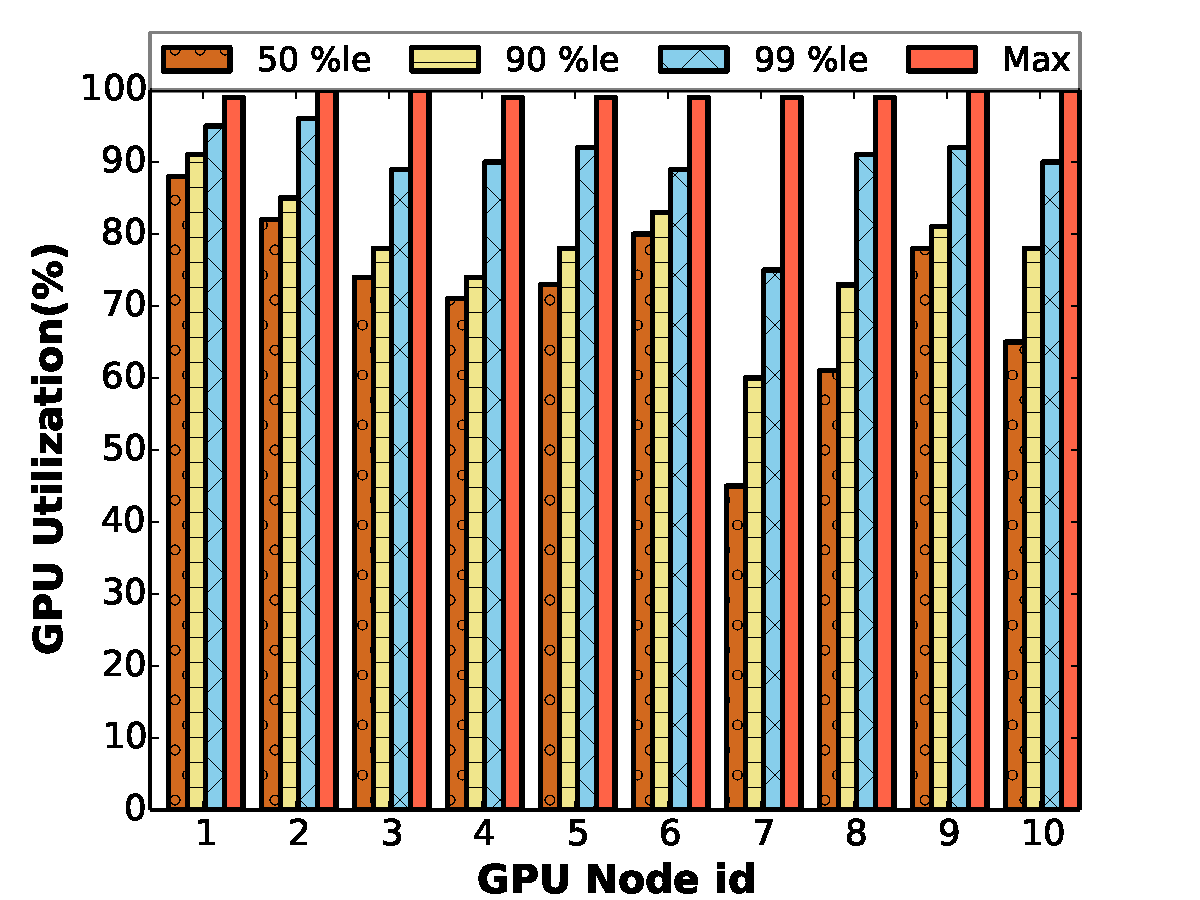
\includegraphics[width=1.1\linewidth]{results/app1-peak.pdf}
  \caption{Application-Mix-1}
  \label{fig:app1-pcp}
\end{subfigure}
\begin{subfigure}[b]{.33\textwidth}
  \centering
  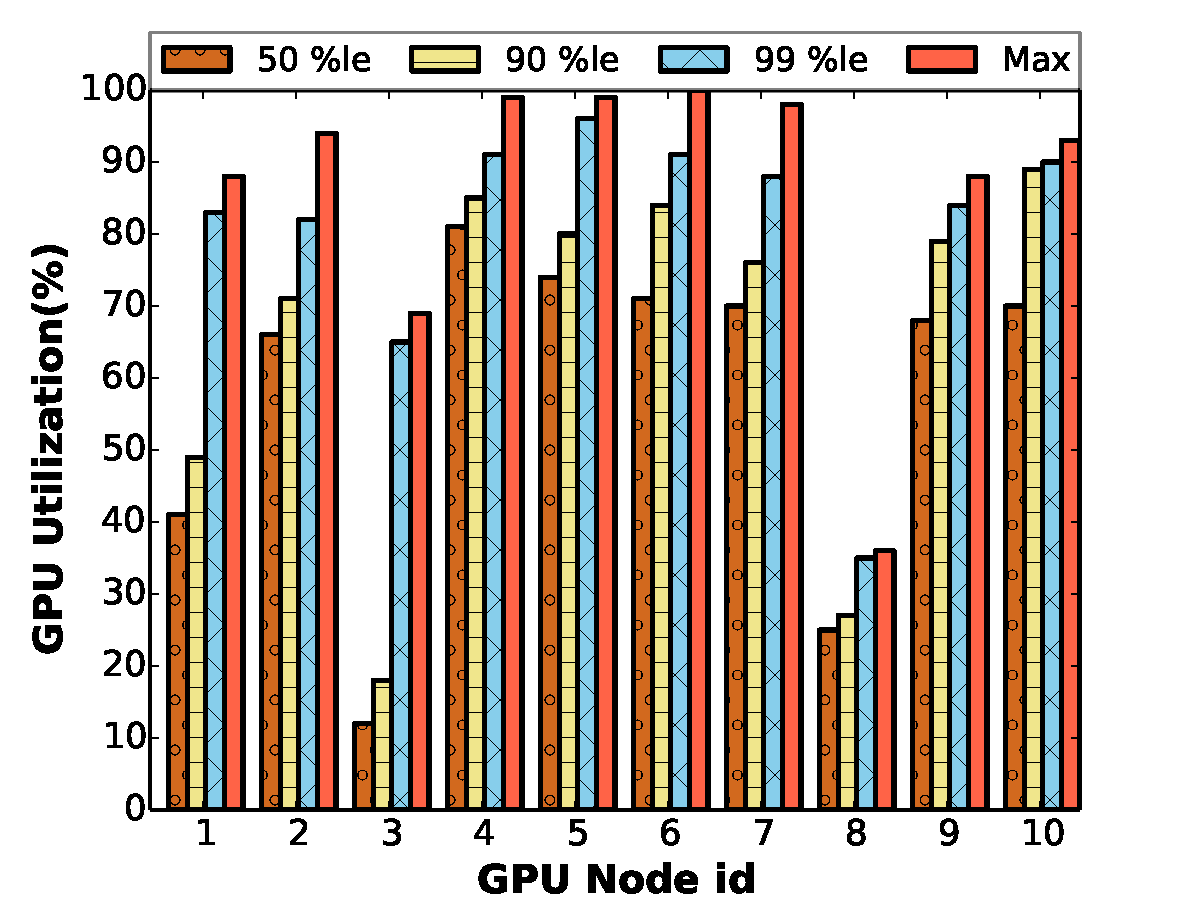
\includegraphics[width=1.1\linewidth]{results/app2-peak.pdf}
  \caption{Application-Mix-2}
  \label{fig:app2-pcp}
\end{subfigure}
\begin{subfigure}[b]{.33\textwidth}
  \centering
  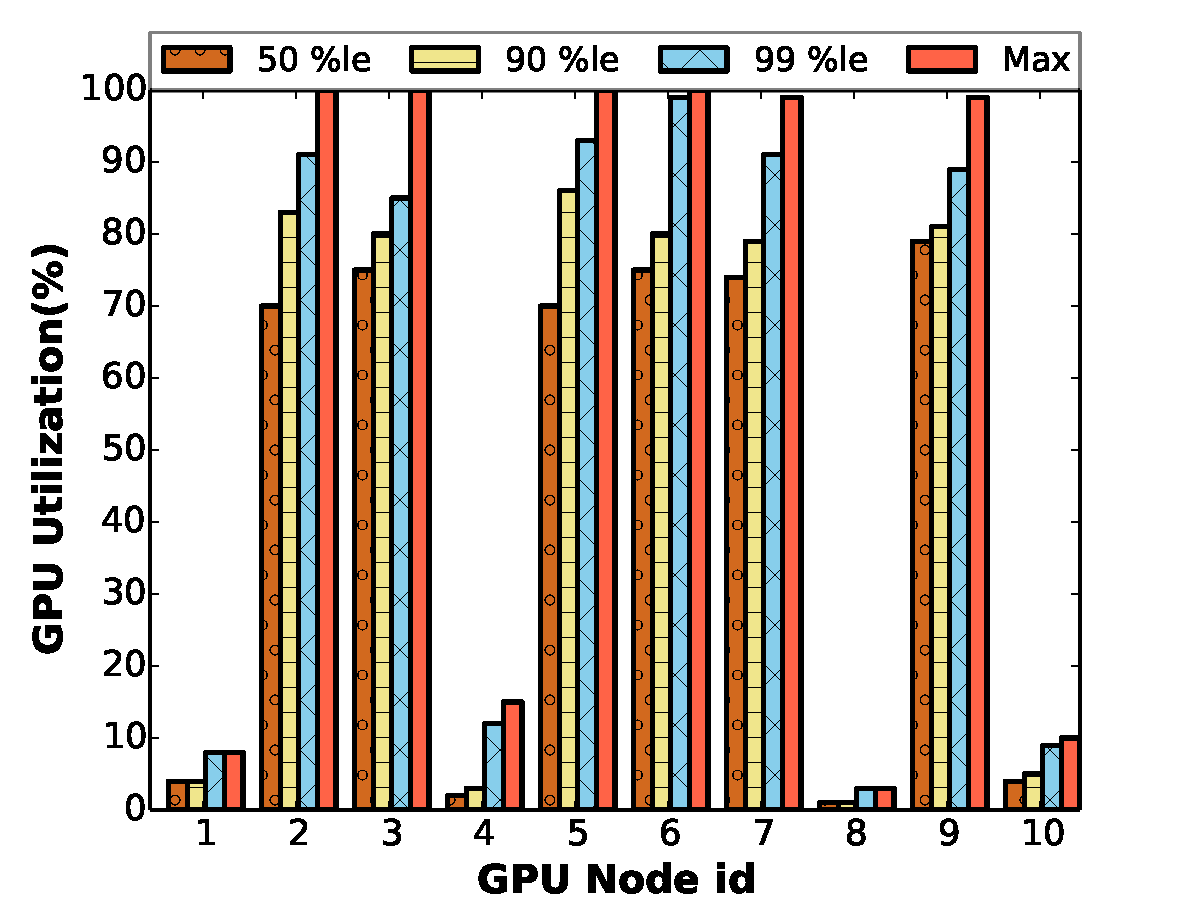
\includegraphics[width=1.1\linewidth]{results/app3-peak.pdf}
  \caption{Application-Mix-3}
  \label{fig:app3-pcp}
\end{subfigure}
\vspace{-6mm}
\caption{50/90/99$^{th}$ percentile \& maximum utilization of GPUs for App-Mixes scheduled using Peak Prediction Scheme.}
\label{fig:pcp}
\end{figure*}

\begin{figure}[tbp!]
\begin{subfigure}[b]{.15\textwidth}
  \centering
  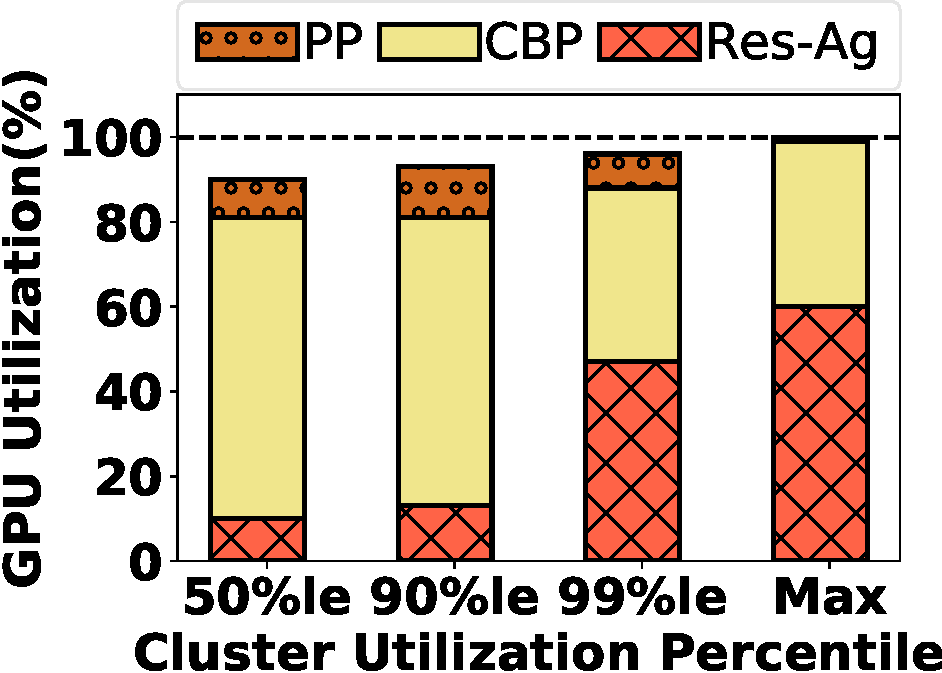
\includegraphics[width=.99\linewidth,height=2cm]{results/app1-avg.pdf}
  \caption{App-Mix-1}
  \label{fig:util1}
\end{subfigure}
\begin{subfigure}[b]{.15\textwidth}
  \centering
  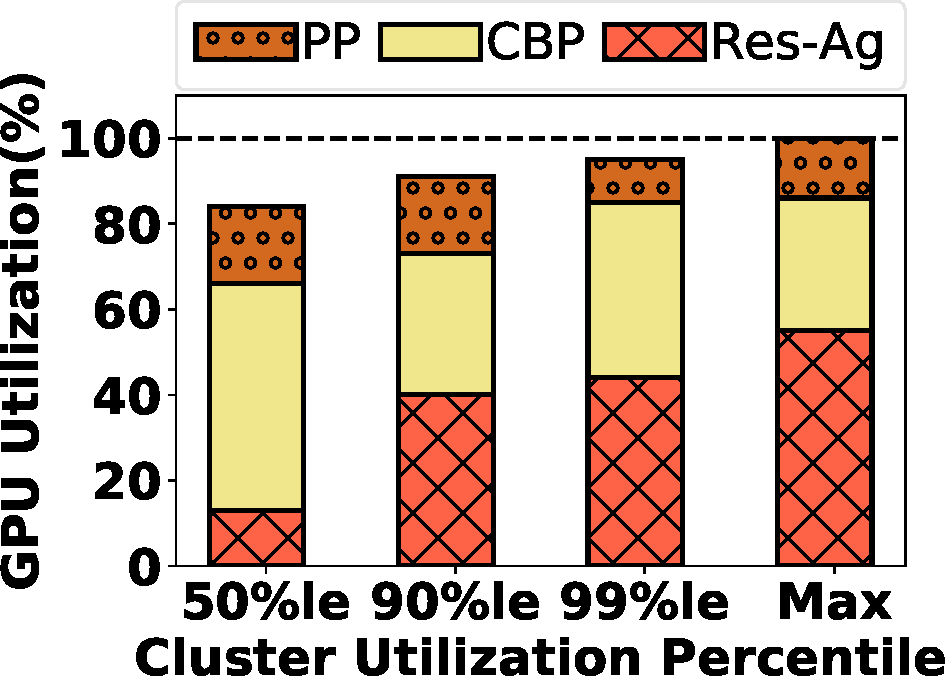
\includegraphics[width=.99\linewidth,height=2cm]{results/app2-avg.pdf}
  \caption{App-Mix-2}
  \label{fig:util2}
\end{subfigure}
\begin{subfigure}[b]{.15\textwidth}
  \centering
  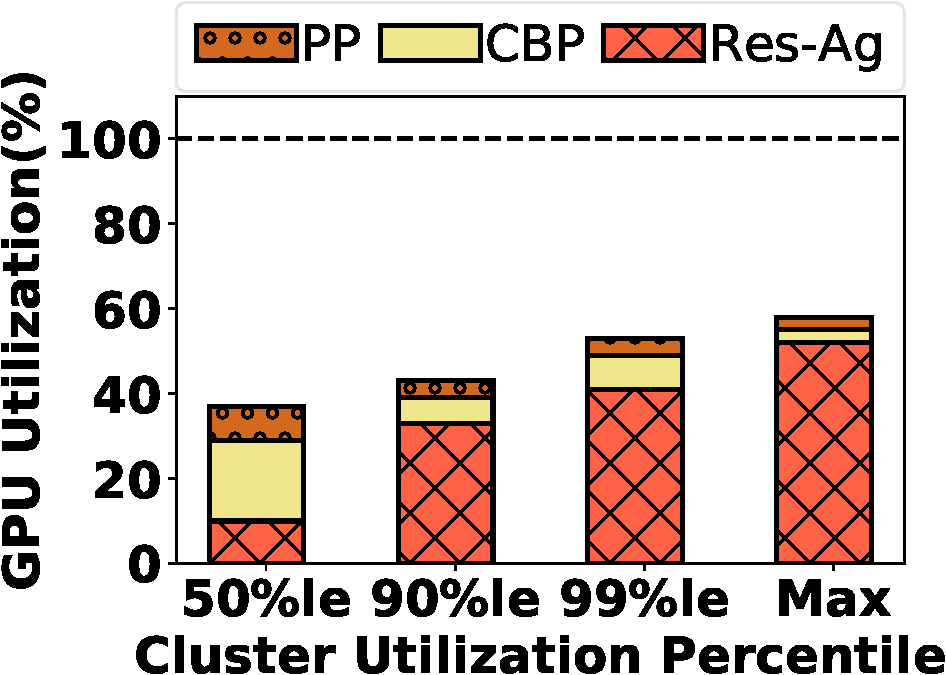
\includegraphics[width=.99\linewidth,height=2cm]{results/app3-avg.pdf}
  \caption{App-Mix-3}
  \label{fig:util3}
\end{subfigure}
\vspace{-3mm}
\caption{Cluster-wide GPU utilization improvements.}
\label{fig:util}
\vspace{-2mm}
\end{figure}

\subsubsection{Container Configuration}

Both the batch and user-facing applications are containerized as pods in \textit{Kubernetes}, and their image is made available in all the GPU nodes beforehand, to avoid any startup latencies. The software configuration is given in Table~\ref{tbl:sw-config} Since these containers are multi-GB and pre-packed with the datasets along with the workloads, the start-up latency depends entirely on the network bandwidth to download the container from a docker-hub or launch from the head-node. To avoid any unprecedented network delays while shipping these containers, we made sure all the nodes had the docker image of the respective workloads in advance. This way, a scheduler can potentially launch the application in any node for the same shipping cost (Typically, the image will be downloaded for the first time (cold start) and then will continue to persist until the container is killed). For application resizing, we used NVIDIA-docker commands to resize the containers before launching the application mixes dynamically. 

Recall from Section \ref{sec:modeling} that, for batch applications we used Rodinia~\cite{che2009rodinia}, HPC and scientific workload suite. Similarly, for latency critical workloads, we used Djinn \& Tonic workload suite~\cite{hauswald2015djinn} which has several DNN inference queries using Tensorflow(TF) on GPUs through Keras libraries for execution. We configured TF's GPU configuration knobs to allow incremental memory growth for the DNN inference queries.  We capture the inter-arrival pattern of the Alibaba trace which is representative of the datacenter workload. We incorporate this inter-arrival pattern in our launch sequence of jobs. The  job sequence comprises of a bin of application-mixes (refer Figure \ref{fig:cov}). 
%\end{itemize}
%\subsubsection{Workload setup}
 




%\subsection{Headnode setup}
%The query interval can be tuned further to improve the accuracy of our peak prediction model at the cost of device overheads due to intrusive monitoring.


